\documentclass[10pt]{article}
\usepackage[utf8]{inputenc}
\usepackage[doublespacing]{setspace}
\usepackage{textcomp}
\usepackage{amsmath,amssymb,amsthm}
\usepackage{fancyhdr}
\usepackage{lastpage}
\usepackage[]{hyperref}
\usepackage[pdftex]{graphicx}
\usepackage{ctex}
\usepackage{booktabs}
\usepackage{subfigure}
\usepackage{titlesec}
\usepackage{listings}
\usepackage{enumerate}
\usepackage{bm}
\usepackage{float}
%\allowdisplaybreaks
\renewcommand{\contentsname}{\centerline{Contents}}
\pagestyle{fancy}
\author{D}
\def\name{D}
\lhead{Time Series Methods}
\chead{}
\rhead{\name}
\cfoot{-\space\thepage\space-}
\newtheorem{exer}{\bm{$Exercise$}}
\newtheorem{prob}{\bm{$Problem$}}
\newtheorem{bonus}{\bm{$Bonus\;Problem$}}
\newcommand{\tabincell}[2]{\begin{tabular}{@{}#1@{}}#2\end{tabular}}
\CTEXoptions[today=old]

\begin{document}

\title{Assignment One}
\date{\today}
\maketitle
\thispagestyle{fancy}
\thispagestyle{fancy}

\begin{prob}
\end{prob}
\begin{enumerate}[1)]
\vspace{3mm}

\item
The differences between a time series $X_{t_1}$, $X_{t_2}$, ..., $X_{t_n}$ and i.i.d. random variables $Y_1$, $Y_2$, ..., $Y_n$ are
\subitem
a) $X_{t_1}$, $X_{t_2}$, ..., $X_{t_n}$ can depend on each other; $Y_1$, $Y_2$, ..., $Y_n$ are all independent.
\subitem
b) $X_{t_1}$, $X_{t_2}$, ..., $X_{t_n}$ are not identical, with possibly different variances; $Y_1$, $Y_2$, ..., $Y_n$ are identical.
\subitem
c) $X_{t_1}$, $X_{t_2}$, ..., $X_{t_n}$ can depend on the observation time, so the order of observation matters; $Y_1$, $Y_2$, ..., $Y_n$ do not depend on the observation time, so the order of observation does not matter.
\vspace{3mm}

\item
The properties of the strong white noise with random variables $W_t$, $t$ = $t_1$, $t_2$, ..., $t_n$ are
\subitem
a) $W_t$ has zero mean, i.e. $\mathbb{E}[W_t] = 0$ for all t.
\subitem
b) The sequence of $W_t$ is homoscedastic and the variance is finite, i.e. $VAR[W_t] = \sigma^2_W < \infty$ for all t.
\subitem
c) $W_{t_1}$, $W_{t_2}$, ..., $W_{t_n}$ are independent, which implies uncorrelation, i.e. $CORR[W_t, W_{t'}] = 0$ whenever $t \neq t'$.
\vspace{3mm}

\item
An M3-competition time series can be in a damped trend. In this example, it is common that the early trend of an M3 series is fixed but gradually dies out.\footnote{ Gardner, E. S., \& McKenzie, E. (2009). \textit{Why the damped trend works}. 1, 7, 12.}
\vspace{3mm}

\item
An significantly large seasonal increase in December retail sales in New South Wales due to Christmas shopping can be in an end-and-peak cycle. In this example, the magnitude of the seasonal component increases over time.\footnote{ Australian Bureau of Statistics. (2017). \textit{Time series analysis: the basics}. Retrieved from https://www.abs.gov.au/websitedbs/d3310114.nsf/home/time+series+analysis:+the+basics/.}

\end{enumerate}
\vspace{3mm}

\begin{prob}
\end{prob}
\begin{enumerate}[1)]
\vspace{3mm}

\item
\begin{proof}
Let X be a numerically valued random variable with expected value $\mu = \mathbb{E}[X]$. Then the variance of X, denoted by $VAR[X]$, is
\begin{equation}
VAR[X]=\mathbb{E}[(X-\mu)^2].
\end{equation}
Then, we have
\begin{align*}
Right\;side&=(\mathbb{E})^2+\mathbb{E}[(X-\mu)^2]\\
&=(\mathbb{E}[X])^2+\mathbb{E}[X^2-2X\mu+\mu^2]\\
&=(\mathbb{E}[X])^2+\mathbb{E}[X^2]-2\mathbb{E}[\mu]\mathbb{E}[X]+\mathbb{E}[\mu^2]\\
&=(\mathbb{E}[X])^2+\mathbb{E}[X^2]-2\mu\mathbb{E}[X]+\mu^2\\
&=(\mathbb{E}[X])^2+\mathbb{E}[X^2]-2(\mathbb{E}[X])^2+(\mathbb{E}[X])^2\\
&=\mathbb{E}[X^2]
\end{align*}
\end{proof}
\vspace{3mm}

\item
\begin{proof}
Let X and Y be random variables. The covariance, denoted by $COV[X,Y]$, is
\begin{equation}
COV[X,Y]=\mathbb{E}[(X-\mu[X])(Y-\mu[Y])].
\end{equation}
Then, we have
\begin{align*}
Left\;side&=\mathbb{E}[(X+Y)^2]-(\mathbb{E}[X]+\mathbb{E}[Y])^2\\
&=\mathbb{E}[X^2]+2\mathbb{E}[XY]+\mathbb{E}[Y^2]-(\mathbb{E}[X])^2-2\mathbb{E}[X]\mathbb{E}[Y]-(\mathbb{E}[Y])^2\\
&=VAR[X]+VAR[Y]+2\mathbb{E}[XY]-2\mathbb{E}[X]\mathbb{E}[Y]\\
&=VAR[X]+VAR[Y]+2(\mathbb{E}[XY]-\mu[Y]\mathbb{E}[X]-\mu[X]\mathbb{E}[Y]+\mu[X]\mu[Y])\\
&=VAR[X]+VAR[Y]+2(\mathbb{E}[XY-X\mu[Y]-Y\mu[X]+\mu[X]\mu[Y]]\\
&=VAR[X]+VAR[Y]+2COV[X,Y]
\end{align*}
\end{proof}
\vspace{3mm}

\item
\begin{proof}
According to the definitions given, we have
\begin{align*}
Left\;side&=\mathbb{E}[\frac{1}{n-1}(X_n-X_1)]\\
&=\frac{1}{n-1}\mathbb{E}[\delta+X_{n-1}+W_n-X_1]\\
&=\frac{1}{n-1}\mathbb{E}[\delta+\delta+X_{n-2}+W_{n-1}+W_n-X_1]\\
&...\\
&=\frac{1}{n-1}\mathbb{E}[(n-1)\delta+X_1+W_n+W_{n-1}+...+W_2-X_1]\\
&=\frac{1}{n-1}\mathbb{E}[(n-1)\delta]+\mathbb{E}[W_n+W_{n-1}+...+W_2]\\
&=\frac{n-1}{n-1}\mathbb{E}[\delta]+0\\
&=\mathbb{E}[\delta]\\
&=\delta
\end{align*}
Hence, the drift estimator $\hat{\delta}$ is unbiased.
\end{proof}
\vspace{3mm}

\item
\begin{proof}
\begin{align*}
Left\;side&=VAR[\frac{1}{n-1}(X_n-X_1)]\\
&=\frac{1}{(n-1)^2}VAR[X_n-X_1]\\
&=\frac{1}{(n-1)^2}VAR[(n-1)\delta+W_n+W_{n-1}+...+W_2+X_1-X_1]\\
&=\frac{1}{(n-1)^2}(VAR[\delta]+VAR[W_n]+VAR[W_{n-1}]+...+VAR[W_2])\\ % Comment: what about COV?
&=\frac{1}{(n-1)^2}(0+\sum_i^{n-1}\sigma^2_W)\\
&=\frac{(n-1)\sigma^2_W}{(n-1)^2}\\
&=\frac{\sigma^2_W}{n-1}
\end{align*}
\end{proof}

\end{enumerate}
\vspace{3mm}

\begin{prob}
\end{prob}
\begin{enumerate}[1)]
\vspace{3mm}

\item
R codes:
\lstinputlisting{p31a.R} % Comment: need uniform
\begin{figure}[H]
  \centering
  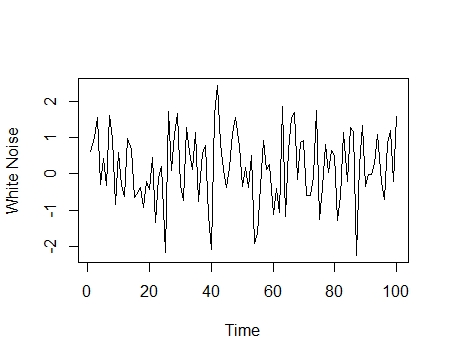
\includegraphics[width=8cm,height=5cm]{p31a.jpeg}
  \caption{Time series with 100 observations of white noise}
\end{figure}
\vspace{3mm}

\item
R codes:
\lstinputlisting{p32a.R}
\begin{figure}[H]
  \centering
  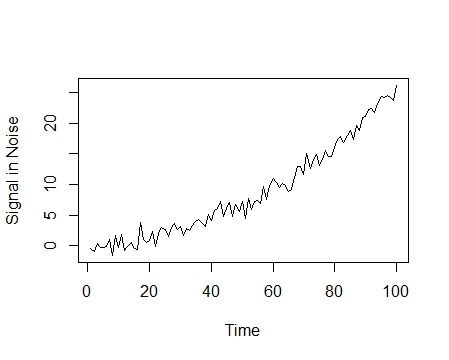
\includegraphics[width=8cm,height=5cm]{p32a.jpeg}
  \caption{Time series with 100 observations of white noise and one signal}
\end{figure}

\end{enumerate}
\vspace{3mm}

\begin{prob}
\end{prob}
\begin{enumerate}[1)]
\vspace{3mm}

\item
R codes:
\lstinputlisting{p41a.R} % Comment: start = c(1959, 251)
\begin{figure}[H]
  \centering
  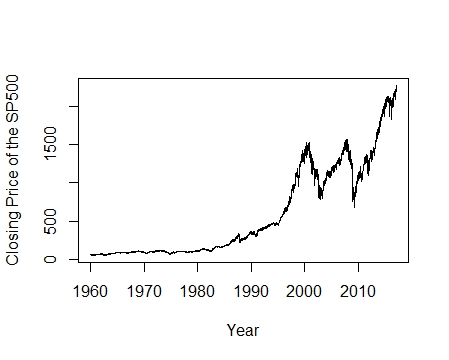
\includegraphics[width=8cm,height=5cm]{p41a.jpeg}
  \caption{Time series with 14349 observations of closing prices of the SP500}
\end{figure}
\vspace{3mm}

\item
Yes, I may transform the data into the logarithmic form, which makes the drift and the volatility both decreased to better fit a random walk model.
\vspace{3mm}

\item
For the original data, the drift is 0.1518637 and the volatility is 8.94192.\\
For the data in the logarithmic form, the drift is 0.0002523836 and the volatility is 0.01007269.\\
R codes
\lstinputlisting{p43a.R}
\vspace{3mm}

\item
R codes:
\lstinputlisting{p44a.R} % Comment: 50 - why?, frequency = 251
\begin{figure}[H]
  \centering
  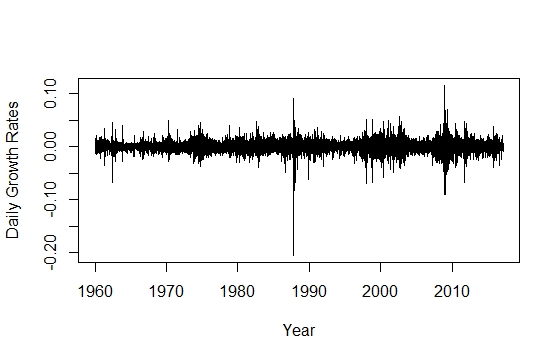
\includegraphics[width=8cm,height=5cm]{p44a.jpeg}
  \caption{Time series with 14348 observations of daily growth rates of prices of the SP500}
\end{figure}
\begin{figure}[H]
  \centering
  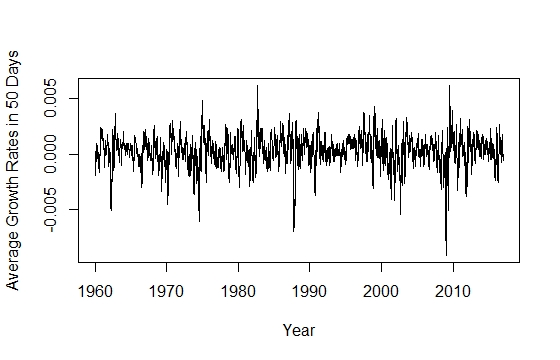
\includegraphics[width=8cm,height=5cm]{p44b.jpeg}
  \caption{Time series with 14248 observations of average growth rates in 50 days of prices of the SP500}
\end{figure}

\end{enumerate}
\vspace{3mm}

\begin{bonus}
\end{bonus}
\vspace{3mm}

Bias:
\begin{align*}
\mathbb{E}[X_{n+m}-\hat{X}_{n+m}]&=\mathbb{E}[X_n+(n-m)\delta+(n-m)W_n-X_n+m\hat{\delta}]\\ % Comment: X_n+m\delta+\sum^{m}_{i=n+1}W_i-X_n-m\hat{\delta}
&=\mathbb{E}[(n-m)\delta+(n-m)W_n+\frac{m}{n-1}(x_n-X_1)]\\
&=\mathbb{E}[(n-m)\delta+(n-m)W_n+\frac{m}{n-1}[(n-1)\delta+(n-1)W_n]]\\
&=\mathbb{E}[(n-m)\delta+(n-m)W_n+m\delta+mW_n]\\
&=\mathbb{E}[n\delta+nW_n]\\
&=n\delta
\end{align*}

Variance:
\begin{align*}
VAR[\hat{X}_{n+m}]&=VAR[X_n+m\hat{\delta}]\\
&=VAR[X_0+n\delta+nW_n+m\hat{\delta}]\\
&=VAR[nW_n+\frac{m}{n-1}(X_n-X_1)]\\
&=VAR[nW_n+m\delta+mW_n]\\
&=VAR[(n+m)W_n]\\
&=(n+m)^2\sigma^2_W
\end{align*}

Mean square error\footnote{ Dunker, F. (2019). \textit{Lecture notes in time series methods}. Unpublished manuscript.}:
\begin{align*}
\mathbb{E}[(X_{n+m}-\hat{X}_{n+m})^2]&=(\mathbb{E}[X_{n+m}]-\hat{X}_{n+m})^2+VAR[X_{n+m}-\hat{X}_{n+m}]\\
&=\mathbb{E}[(X_n+m\delta+\sum^{n+m}_{t=n+1}W_t-X_n-m\delta)]^2\\
&=\mathbb{E}[(\sum^{n+m}_{t=n+1}W_t)^2],\;\mathbb{E}[\sum W_t]=0\\
&=VAR[\sum^{n+m}_{t=n+1}W_t]\\
&=\sum^{n+m}_{t=n+1}VAR[W_t]\\
&=m\sigma^2_W
\end{align*}

\end{document}
